\documentclass[12pt]{extarticle}
\usepackage{phys440}

\title{PHYS440 - Homework 1+2}
\author{John Hurst}
\date{March 2024}

\begin{document}
\maketitle

%%%%%%%%%%%%%%%%%%%%%%%%%%%%%%%%%%%%%%%%%%%%%%%%%%%%%%%%%%%%%%%%%%%%%%%%%%%%%%%%%%%%%%%%%%%%%%%%%%%%
\question{1}{Bell-state realization and correlation measurement on \textit{IBM Quantum} (12 marks)

The \textit{Qiskit} textbook chapter on Multiple Qubits and Entangled States explains how to generate the entangled two qubit state
\begin{equation}\label{eq:phiplus}
\ket\Phi^{+} = \istwo(\ket{00} + \ket{11})
\end{equation}
and gives the creation of the Bell state
\begin{equation}\label{eq:psiplus}
\ket\Psi^{+} = \istwo(\ket{01} + \ket{10})
\end{equation}
as an exercise.
Read this/remind yourself of the relevant material.
Furthermore, read up of how to perform measurements of $Z_0=\idone\otimes Z$ and $Z_1=Z\otimes\idone$
to find the correlator $\langle Z_1Z_0\rangle = P_{00}+P_{11}-P_{01}-P_{10}$.
Use this preparation to answer the following questions.
\begin{enumerate}[(i)]
\item Design the quantum circuits that, starting from the two-qubit state $\ket{00}$, create the remaining two Bell states
\begin{equation}\label{eq:phiminus}
\ket\Phi^{-} = \istwo(\ket{00} - \ket{11})
\end{equation}
\begin{equation}\label{eq:psiminus}
\ket\Psi^{-} = \istwo(\ket{01} - \ket{10})
\end{equation}
Show (by using matrix representations of the quantum gates) that the circuits that you have designed indeed yield the Bell states are their output.
Submit the circuit diagrams and state-vector simulations from \textit{IBM Quantum} as part of your solution.
\item Consider the two operators $X_0=\idone\otimes X$ and $X_1=X\otimes\idone$.
Design the circuits that allow you to measure
$\langle \Phi^{+}|X_1X_0|\Phi^{+}\rangle$, where $\ket{\Phi^{+}}$ is defined in Eq.~\eqref{eq:phiplus}.
Run the circuit first on the simulator and then on one of the available quantum processors.
Discuss the result of your experiment.
Submit screenshots of your \textit{IBM Quantum} jobs as part of your solution.
\end{enumerate}
}

\begin{enumerate}[(i)]
\item There are a number of different circuits possible for each Bell state.
The attached Mathematica notebook shows each Bell state created with
certain specific simple circuits using H, CNOT, NOT and Z gates.

I have run circuits for all four Bell states on the IBM quantum simulator.
Screenshots are below:

\begin{figure}[H]
\centering
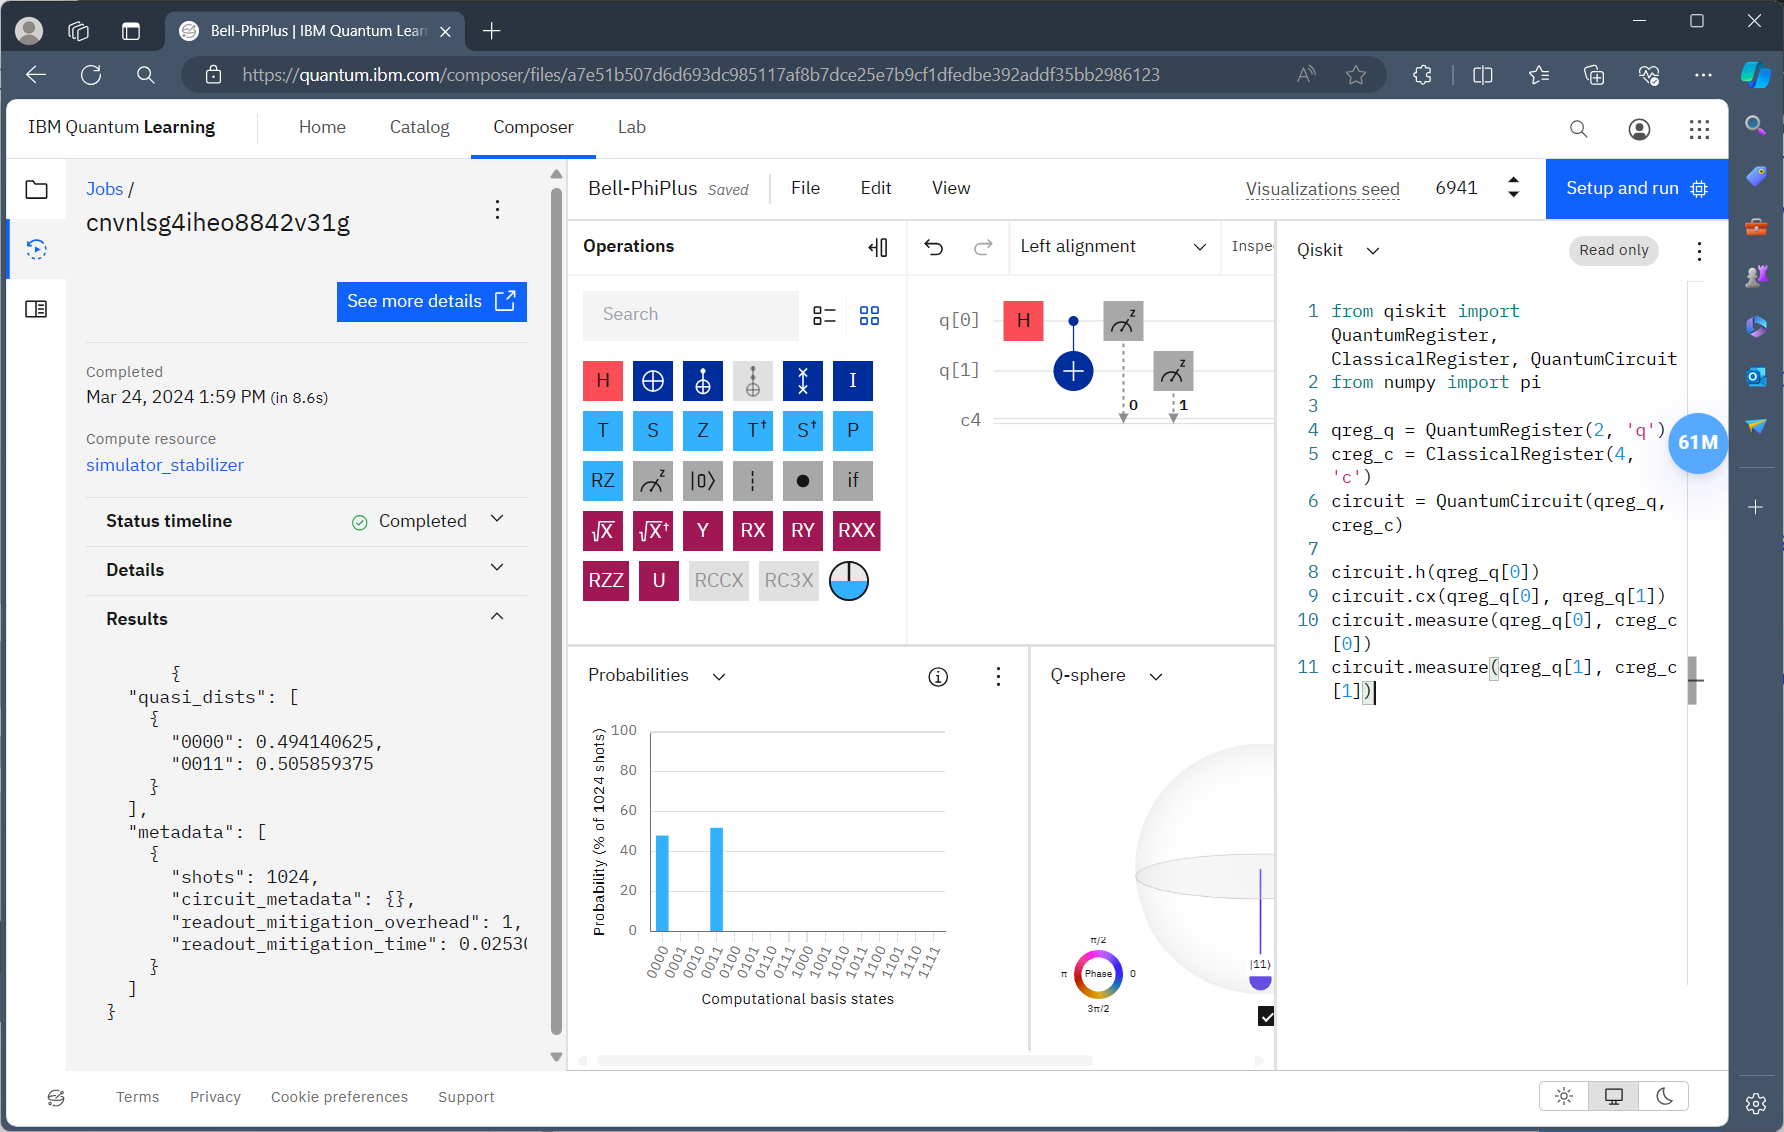
\includegraphics[width=0.80\textwidth]{images/Bell-PhiPlus-IBM-Quantum.png}
\caption{Bell state $\ket{\Phi^{+}}$ on IBM Quantum}
\end{figure}
\begin{figure}[H]
\centering
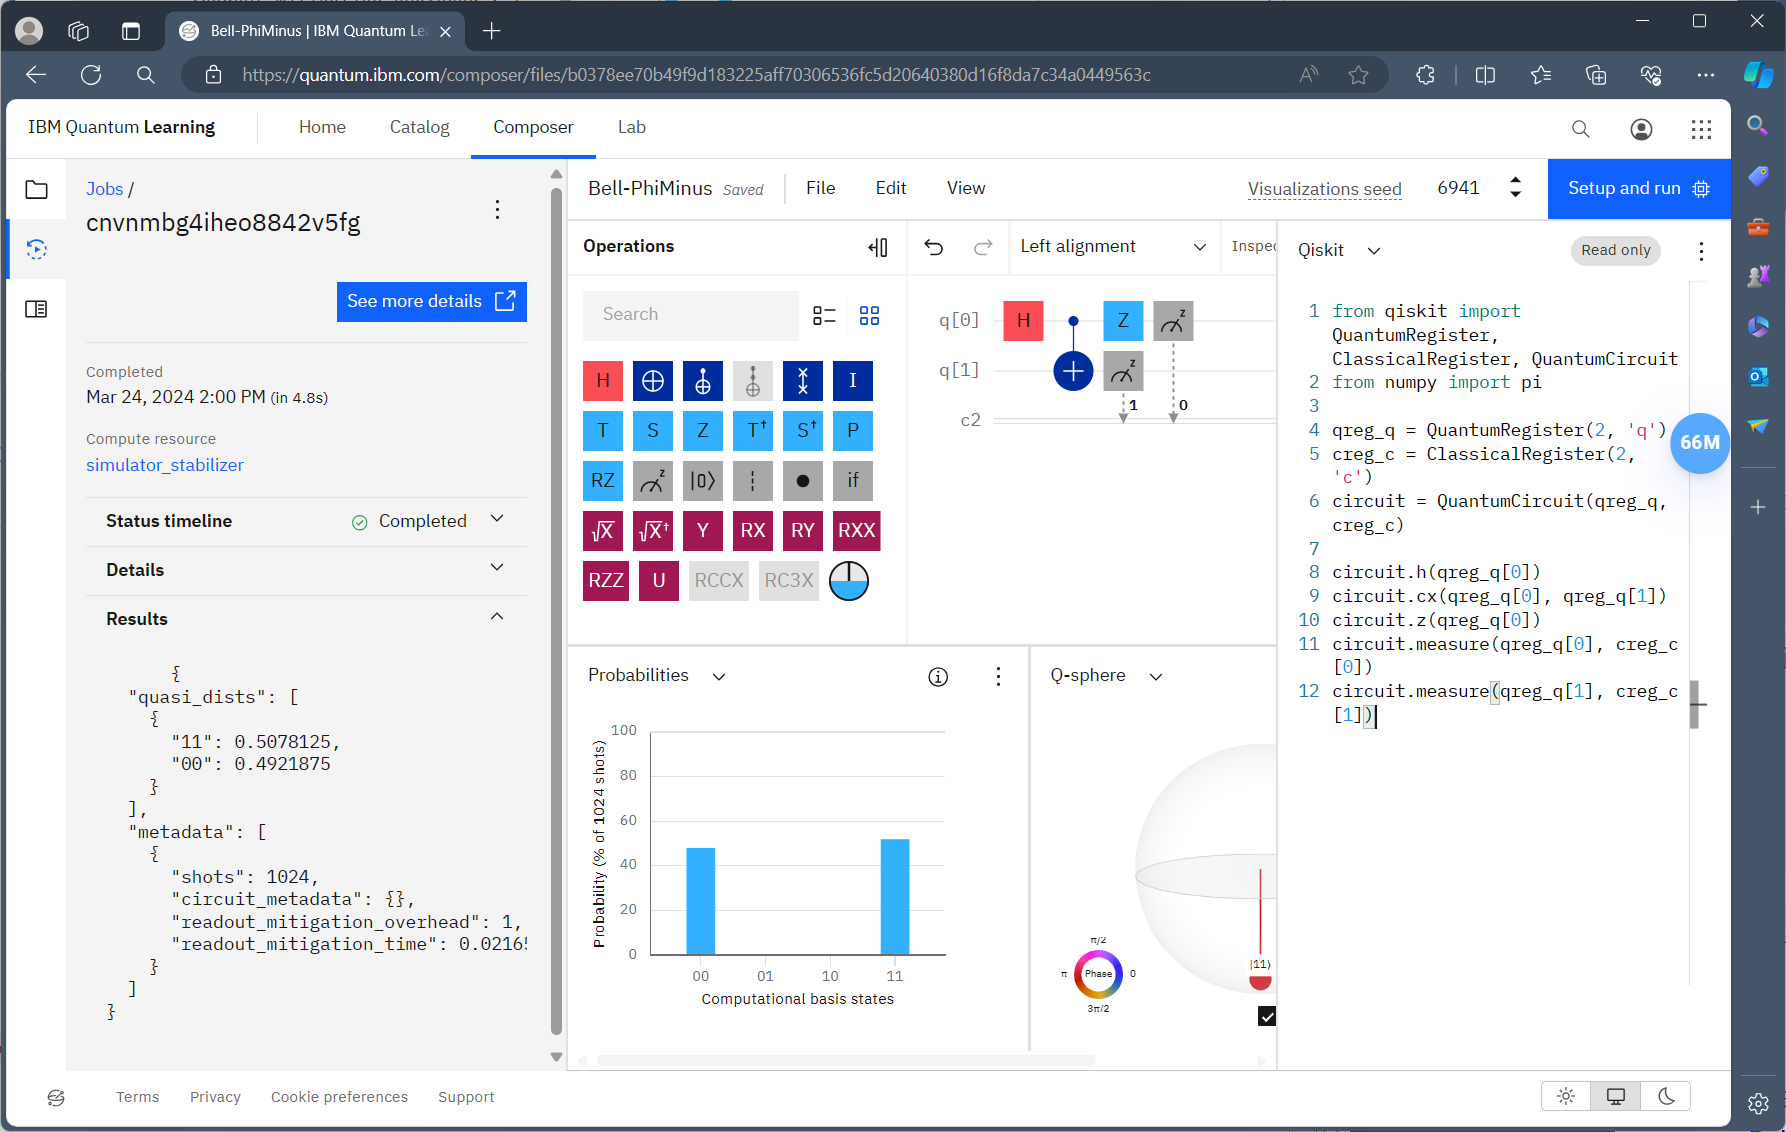
\includegraphics[width=0.80\textwidth]{images/Bell-PhiMinus-IBM-Quantum.png}
\caption{Bell state $\ket{\Phi^{-}}$ on IBM Quantum}
\end{figure}
\begin{figure}[H]
\centering
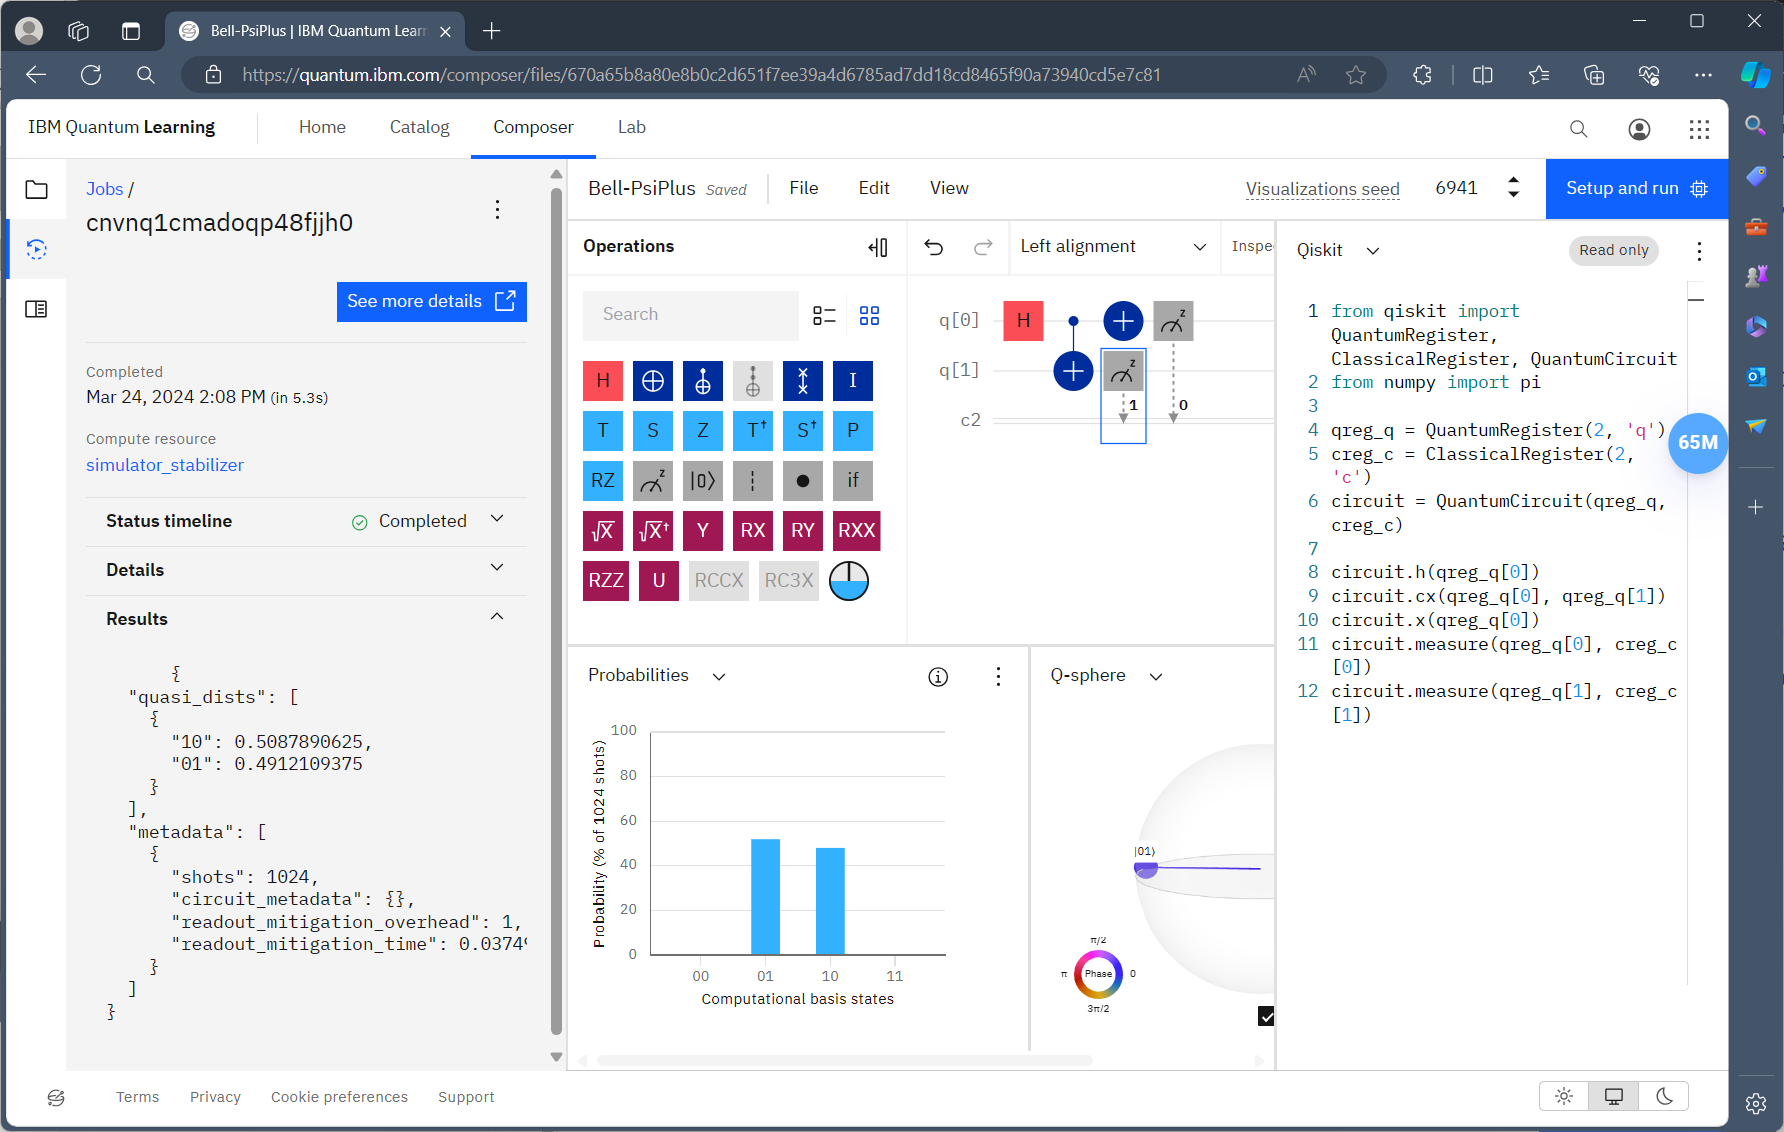
\includegraphics[width=0.80\textwidth]{images/Bell-PsiPlus-IBM-Quantum.png}
\caption{Bell state $\ket{\Psi^{+}}$ on IBM Quantum}
\end{figure}
\begin{figure}[H]
\centering
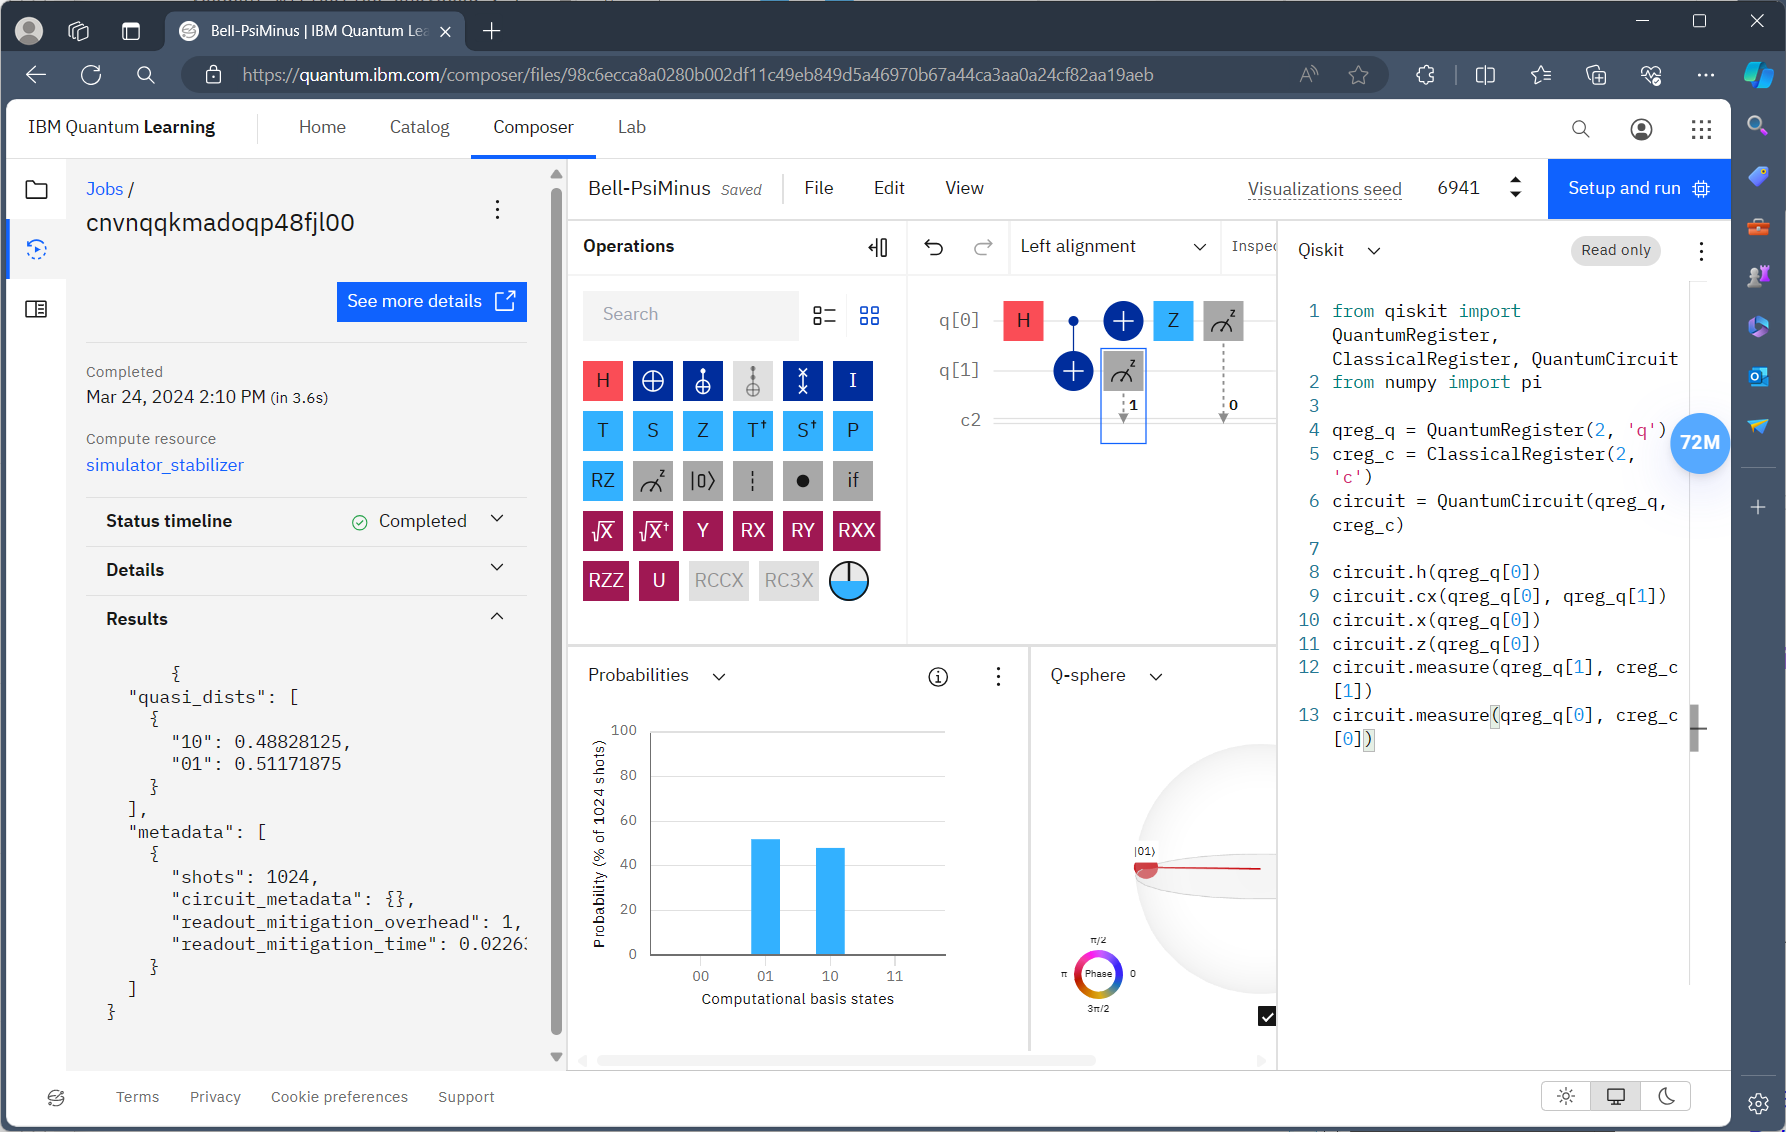
\includegraphics[width=0.80\textwidth]{images/Bell-PsiMinus-IBM-Quantum.png}
\caption{Bell state $\ket{\Psi^{-}}$ on IBM Quantum}
\end{figure}

I've also run these circuits locally using the Basic provider in the Qiskit Python library:
\begin{footnotesize}
\begin{lstlisting}[language=Python]
... # other imports
from qiskit import  ClassicalRegister, QuantumCircuit, QuantumRegister
from qiskit.providers.basic_provider import BasicProvider
from qiskit.primitives import BackendSampler

# argument parsing code omitted

qreg_q = QuantumRegister(2, 'q')
creg_c = ClassicalRegister(2, 'c')
circuit = QuantumCircuit(qreg_q, creg_c)

circuit.h(qreg_q[0])
circuit.cx(qreg_q[0], qreg_q[1])
if args.psiplus or args.psiminus:
    circuit.x(qreg_q[0])
if args.phiminus or args.psiminus:
    circuit.z(qreg_q[0])
circuit.measure(qreg_q[0], creg_c[0])
circuit.measure(qreg_q[1], creg_c[1])

if args.filename:
    with open(args.filename, 'w') as f:
        circuit.draw('mpl', filename=args.filename)

backend = BasicProvider().get_backend('basic_simulator')
sampler = BackendSampler(backend)
job = sampler.run(circuit, shots=args.shots)
result = job.result()
dists = {'{:02b}'.format(int(k)): v
         for k, v in result.quasi_dists[0].items()}
for k in sorted(dists.keys()):
    print(f'{k}: {dists[k]:.4f}')
\end{lstlisting}
\end{footnotesize}

This produces output such as:
\begin{footnotesize}
\begin{lstlisting}
$ bin/homework12_q1i.py --phiplus --filename=images/phiplus.png
00: 0.5010
11: 0.4990
$ bin/homework12_q1i.py --phiminus --filename=images/phiminus.png
00: 0.5078
11: 0.4922
$ bin/homework12_q1i.py --psiplus --filename=images/psiplus.png
01: 0.4951
10: 0.5049
$ bin/homework12_q1i.py --psiminus --filename=images/psiminus.png
01: 0.4805
10: 0.5195
\end{lstlisting}
\end{footnotesize}

And also these circuit images:
\begin{figure}[H]
\centering
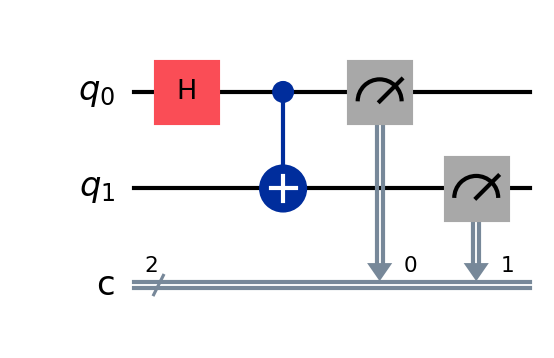
\includegraphics[width=0.50\textwidth]{images/phiplus.png}
\caption{Bell state $\ket{\Phi^{+}}$ on local simulator}
\end{figure}
\begin{figure}[H]
\centering
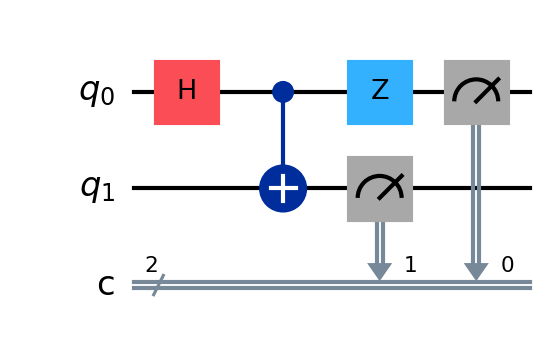
\includegraphics[width=0.50\textwidth]{images/phiminus.png}
\caption{Bell state $\ket{\Phi^{-}}$ on local simulator}
\end{figure}
\begin{figure}[H]
\centering
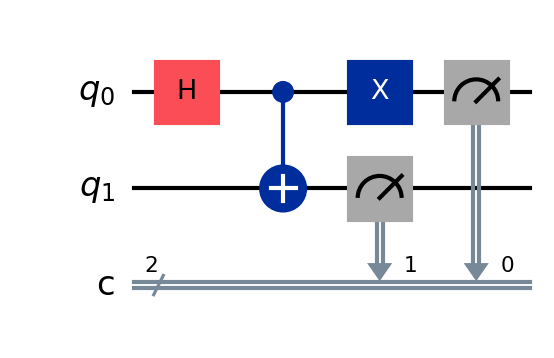
\includegraphics[width=0.50\textwidth]{images/psiplus.png}
\caption{Bell state $\ket{\Psi^{+}}$ on local simulator}
\end{figure}
\begin{figure}[H]
\centering
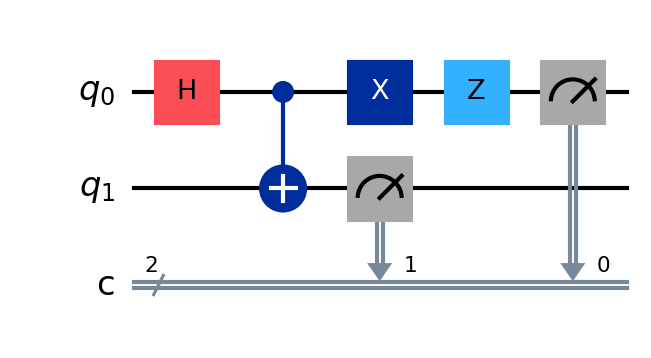
\includegraphics[width=0.50\textwidth]{images/psiminus.png}
\caption{Bell state $\ket{\Psi^{-}}$ on local simulator}
\end{figure}

\item We can compute $X_0$ and $X_1$ and the correlator as:
\begin{align*}
X_0 & = \idone\otimes X = \begin{pmatrix}1&0\\0&1\end{pmatrix}\otimes\begin{pmatrix}0&1\\1&0\end{pmatrix} = \begin{pmatrix}0&1&0&0\\1&0&0&0\\0&0&0&1\\0&0&1&0\end{pmatrix} \\
X_1 & = X\otimes\idone = \begin{pmatrix}0&1\\1&0\end{pmatrix}\otimes\begin{pmatrix}1&0\\0&1\end{pmatrix} = \begin{pmatrix}0&0&1&0\\0&0&0&1\\1&0&0&0\\0&1&0&0\end{pmatrix} \\
X_1X_0 & = \begin{pmatrix}0&0&1&0\\0&0&0&1\\1&0&0&0\\0&1&0&0\end{pmatrix}\begin{pmatrix}0&1&0&0\\1&0&0&0\\0&0&0&1\\0&0&1&0\end{pmatrix} \\
& = \begin{pmatrix}0&0&0&1\\0&0&1&0\\0&1&0&0\\1&0&0&0\end{pmatrix}
\end{align*}

We can compute $\langle \Phi^{+}|X_1X_0|\Phi^{+}\rangle$ as:
\begin{align*}
\langle \Phi^{+}|X_1X_0|\Phi^{+}\rangle
& = \frac{1}{\sqrt{2}}\begin{pmatrix}1&0&0&1\end{pmatrix}
\begin{pmatrix}0&0&0&1\\0&0&1&0\\0&1&0&0\\1&0&0&0\end{pmatrix}
\frac{1}{\sqrt{2}} \begin{pmatrix}1\\0\\0\\1\end{pmatrix} \\
& = \frac{1}{2}\begin{pmatrix}1&0&0&1\end{pmatrix} \begin{pmatrix}1\\0\\0\\1\end{pmatrix} \\
& = \frac{1}{2}(1+1) \\
& = 1
\end{align*}

(See the attached {\mathematica}
notebook for the a check of this calculation.)

\end{enumerate}

%%%%%%%%%%%%%%%%%%%%%%%%%%%%%%%%%%%%%%%%%%%%%%%%%%%%%%%%%%%%%%%%%%%%%%%%%%%%%%%%%%%%%%%%%%%%%%%%%%%%
\question{2}{Testing Bell's Inequality on \textit{IBM Quantum} (28 marks)

To answer the questions below, it will be useful to first familiarise yourself with the CHSH inequality,
e.g. by reading about it in textbooks and/or the document \textit{A Brief Introduction to Entanglement \& the CHSH inequality} from our \texttt{Lit} folder.
You will also have to make use of the techniques learned from Question 1 above.

Consider the state $\ket{\Psi^{-}} = \istwo(\ket{01}-\ket{10})$ and the following observables
\begin{align*}
A & = Z\otimes \idone \quad ; & A' & = X\otimes \idone \\
B & = \idone \otimes \istwo(X+Z) \quad ; & B' & = \idone \otimes \istwo(X-Z).
\end{align*}

\begin{enumerate}[(i)]
\item Calculate analytically, using the matrix representation of the relevant quantum gates, the following correlators:
\begin{equation}\label{eq:correlators}
\langle \Psi^{-}|AB|\Psi^{-}\rangle, \quad \langle \Psi^{-}|AB' |\Psi^{-}\rangle , \quad \langle \Psi^{-}|A'B|\Psi^{-}\rangle, \quad \langle \Psi^{-}|A'B'|\Psi^{-}\rangle,
\end{equation}
as well as the quantity
\begin{equation}\label{eq:c}
C = \langle \Psi^{-}|AB|\Psi^{-}\rangle - \langle \Psi^{-}|AB' |\Psi^{-}\rangle + \langle \Psi^{-}|A'B|\Psi^{-}\rangle + \langle \Psi^{-}|A'B'|\Psi^{-}\rangle.
\end{equation}
\item Design the four quantum circuits that will allow you to measure the expectation values given in Eq.~\eqref{eq:correlators}.
Submit the circuit diagrams from \textit{IBM Quantum} as part of your solution.
\item Run the circuits on the simulator, evaluate the expectation values from Eq.~\eqref{eq:correlators},
and check whether the CHSH inequality is violated.
Submit screenshots of your \textit{IBM Quantum} jobs as part of your solution.
\item Now run your circuits on one of the available quantum processors and evaluate the expectation values from Eq.~\eqref{eq:correlators} as well as $|C|$,
with $C$ given in Eq.~\eqref{eq:c}.
\item Submit screenshots of your \textit{IBM Quantum} jobs as part of your solution.
\item Comment on your result, discussing specifically whether---and if so, at what level of confidence---it rules out the possibility of a hidden variable theory.
\end{enumerate}
}

% \printbibliography
% \addcontentsline{toc}{section}{References}

\end{document}
